\documentclass{standalone}
\usepackage{tikz}
\begin{document}
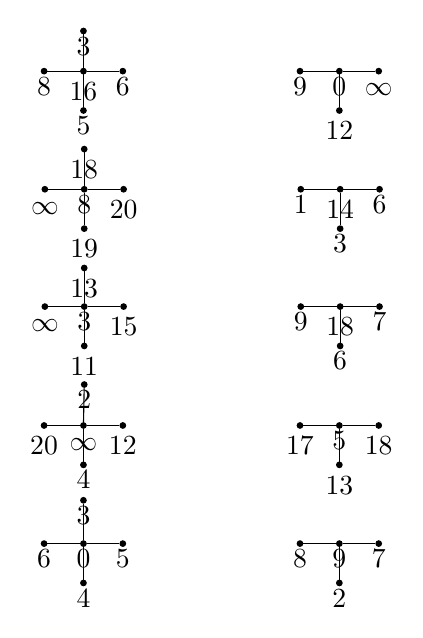
\begin{tikzpicture}[every node/.style={draw, circle, fill=black, minimum size=2pt, inner sep=0pt}]
\node[fill=black, label=below:{\color{black}$8$}] (G1N8) at (3.99,7.00) {};
\node[fill=black, label=below:{\color{black}$16$}] (G1N16) at (4.49,7.00) {};
\node[fill=black, label=below:{\color{black}$6$}] (G1N6) at (4.99,7.00) {};
\node[fill=black, label=below:{\color{black}$5$}] (G1N5) at (4.49,6.50) {};
\node[fill=black, label=below:{\color{black}$3$}] (G1N3) at (4.49,7.51) {};
\node[fill=black, label=below:{\color{black}$9$}] (G1N9) at (7.24,7.00) {};
\node[fill=black, label=below:{\color{black}$0$}] (G1N0) at (7.74,7.00) {};
\node[fill=black, label=below:{\color{black}$\infty$}] (G1Ninf) at (8.24,7.00) {};
\node[fill=black, label=below:{\color{black}$12$}] (G1N12) at (7.74,6.50) {};
\draw (G1N16) -- (G1N8);
\draw (G1N16) -- (G1N6);
\draw (G1N16) -- (G1N5);
\draw (G1N16) -- (G1N3);
\draw (G1N0) -- (G1Ninf);
\draw (G1N0) -- (G1N12);
\draw (G1N0) -- (G1N9);
\node[fill=black, label=below:{\color{black}$\infty$}] (G2Ninf) at (4.00,5.50) {};
\node[fill=black, label=below:{\color{black}$8$}] (G2N8) at (4.50,5.50) {};
\node[fill=black, label=below:{\color{black}$20$}] (G2N20) at (5.00,5.50) {};
\node[fill=black, label=below:{\color{black}$19$}] (G2N19) at (4.50,5.00) {};
\node[fill=black, label=below:{\color{black}$18$}] (G2N18) at (4.50,6.01) {};
\node[fill=black, label=below:{\color{black}$1$}] (G2N1) at (7.25,5.50) {};
\node[fill=black, label=below:{\color{black}$14$}] (G2N14) at (7.75,5.50) {};
\node[fill=black, label=below:{\color{black}$6$}] (G2N6) at (8.25,5.50) {};
\node[fill=black, label=below:{\color{black}$3$}] (G2N3) at (7.75,5.00) {};
\draw (G2N8) -- (G2Ninf);
\draw (G2N8) -- (G2N20);
\draw (G2N8) -- (G2N19);
\draw (G2N8) -- (G2N18);
\draw (G2N14) -- (G2N6);
\draw (G2N14) -- (G2N3);
\draw (G2N14) -- (G2N1);
\node[fill=black, label=below:{\color{black}$\infty$}] (G3Ninf) at (4.00,4.01) {};
\node[fill=black, label=below:{\color{black}$3$}] (G3N3) at (4.50,4.01) {};
\node[fill=black, label=below:{\color{black}$15$}] (G3N15) at (5.00,4.01) {};
\node[fill=black, label=below:{\color{black}$11$}] (G3N11) at (4.50,3.51) {};
\node[fill=black, label=below:{\color{black}$13$}] (G3N13) at (4.50,4.50) {};
\node[fill=black, label=below:{\color{black}$9$}] (G3N9) at (7.25,4.01) {};
\node[fill=black, label=below:{\color{black}$18$}] (G3N18) at (7.75,4.01) {};
\node[fill=black, label=below:{\color{black}$7$}] (G3N7) at (8.25,4.01) {};
\node[fill=black, label=below:{\color{black}$6$}] (G3N6) at (7.75,3.51) {};
\draw (G3N3) -- (G3Ninf);
\draw (G3N3) -- (G3N15);
\draw (G3N3) -- (G3N11);
\draw (G3N3) -- (G3N13);
\draw (G3N18) -- (G3N9);
\draw (G3N18) -- (G3N7);
\draw (G3N18) -- (G3N6);
\node[fill=black, label=below:{\color{black}$20$}] (G4N20) at (3.99,2.50) {};
\node[fill=black, label=below:{\color{black}$\infty$}] (G4Ninf) at (4.49,2.50) {};
\node[fill=black, label=below:{\color{black}$12$}] (G4N12) at (4.99,2.50) {};
\node[fill=black, label=below:{\color{black}$4$}] (G4N4) at (4.49,2.00) {};
\node[fill=black, label=below:{\color{black}$2$}] (G4N2) at (4.50,3.02) {};
\node[fill=black, label=below:{\color{black}$17$}] (G4N17) at (7.24,2.50) {};
\node[fill=black, label=below:{\color{black}$5$}] (G4N5) at (7.74,2.50) {};
\node[fill=black, label=below:{\color{black}$18$}] (G4N18) at (8.24,2.50) {};
\node[fill=black, label=below:{\color{black}$13$}] (G4N13) at (7.74,2.00) {};
\draw (G4Ninf) -- (G4N20);
\draw (G4Ninf) -- (G4N12);
\draw (G4Ninf) -- (G4N4);
\draw (G4Ninf) -- (G4N2);
\draw (G4N5) -- (G4N18);
\draw (G4N5) -- (G4N17);
\draw (G4N5) -- (G4N13);
\node[fill=black, label=below:{\color{black}$6$}] (G5N6) at (3.99,1.00) {};
\node[fill=black, label=below:{\color{black}$0$}] (G5N0) at (4.49,1.00) {};
\node[fill=black, label=below:{\color{black}$5$}] (G5N5) at (4.99,1.00) {};
\node[fill=black, label=below:{\color{black}$4$}] (G5N4) at (4.49,0.50) {};
\node[fill=black, label=below:{\color{black}$3$}] (G5N3) at (4.49,1.55) {};
\node[fill=black, label=below:{\color{black}$8$}] (G5N8) at (7.24,1.00) {};
\node[fill=black, label=below:{\color{black}$9$}] (G5N9) at (7.74,1.00) {};
\node[fill=black, label=below:{\color{black}$7$}] (G5N7) at (8.24,1.00) {};
\node[fill=black, label=below:{\color{black}$2$}] (G5N2) at (7.74,0.50) {};
\draw (G5N0) -- (G5N6);
\draw (G5N0) -- (G5N5);
\draw (G5N0) -- (G5N4);
\draw (G5N0) -- (G5N3);
\draw (G5N9) -- (G5N8);
\draw (G5N9) -- (G5N7);
\draw (G5N9) -- (G5N2);
\end{tikzpicture}
\end{document}
